\section{Měření teplot při vysokých podzvukových rychlostech} \label{sec:mereni-teplot}
    Teplota, jako stavová veličina, je jedním z důležitých parametrů proudění, které jsou sledovány během průmyslových procesů, nebo během provozu strojírenských zařízení, či výzkumných tratí. Její měření je obvykle bezproblémové, hovoříme-li o nízkých rychlostech proudění, nebo případně o kapalinách. Při přechodu do vyšších podzvukových rychlostí plynů (na které je zaměřena tato práce) dochází k nárůstu vlivu jejich stlačitelnosti a určení statické, potažmo stagnační, teploty proudění začíná být problematické. Hranice stlačitelnosti se obvykle uvažuje okolo $\Ma = 0.3$.

    \subsection{Dynamický ohřev}

    Dobrým ukazatelem míry vlivu stlačitelnosti proudění na měření teploty je poměr statické a stagnační teploty, který lze odvodit z energetické rovnice při uvažování adiabatického výtoku z nádoby o klidových parametrech $h_0$, $T_0$ a $u_0 = 0 \Unit{\frac{m}{s}}$ do obecného místa s parametry $h$, $T$ a $u$:

    \begin{align}
        h_0 &= h + \frac{u^2}{2} \\
        h &= c_p T \\
        c_p T_0 &= c_p T + \frac{u^2}{2} \\
        T_0 &= T + \frac{u^2}{2 c_p} = T + \frac{u^2}{2 c_p} \frac{a^2}{a^2} \label{eq:T0} \\
        a &= \sqrt{\kappa r T} \\
        c_p &= \frac{\kappa r}{\kappa - 1} \\
        T_0 &= T \brac{1 + \frac{\kappa - 1}{2} \frac{u^2}{a^2}} \\
        \Ma &= \frac{u}{a} \\
        \frac{T}{T_0} &= \frac{1}{1 + \frac{\kappa - 1}{2} \Ma ^2}  \label{eq:pomer-T-T0}
    \end{align}

    \noindent kde $h \unit{\frac{J}{kg}}$ je měrná entalpie, $u \unit{\frac{m}{s}}$ je rychlost proudění, $T \unit{K}$ je termodynamická teplota, $c_p \unit{\frac{J}{kg K}}$ je měrná tepelná kapacita za konstantního tlaku, $a \unit{\frac{m}{s}}$ je rychlost zvuku, $\kappa \unit{1}$ je Poissonova konstanta, $r \unit{\frac{J}{kg K}}$ je měrná plynová konstanta a  $\Ma \unit{1}$ je Machovo číslo. Dolní index $0$ označuje stagnační parametry.

    Ze Vztahu \ref{eq:pomer-T-T0} je patrné, že při nulové rychlosti proudění ($\Ma = 0$) bude statická teplota rovna teplotě stagnační, neboli klidové. Dosažením rychlosti zvuku ($\Ma = 1$) klesne poměr na hodnotu $\frac{1}{1+\frac{\kappa - 1}{2}}$, což pro vzduch odpovídá $0.83$ při uvažování $\kappa = 1.4$. Při $\Ma = 0.3$ (zmiňovaná mez stlačitelnosti) tvoří v statická teplota $98.2 \Unit{\%}$ stagnační teploty, zanedbáním dynamické teploty bychom se tak dopustili v tomto případě $1.8\%$ chyby. Chybě $2.5 \Unit{\%}$ pak odpovídá Machovo číslo $0.358$.

    \clearpage

    Člen $\frac{u^2}{2 c_p}$ v Rovnici $\ref{eq:T0}$ je nazýván dynamická teplota (ačkoliv se o teplotu nejedná) a je projevem stlačitelnosti proudění. Jeho průběh v závislosti na Machově čísle je společně s poměrem $\frac{T}{T0}$ vyznačen na Obrázku \ref{fig:pomer-T-T0}.

    \begin{figure}[ht!]
        \centering
        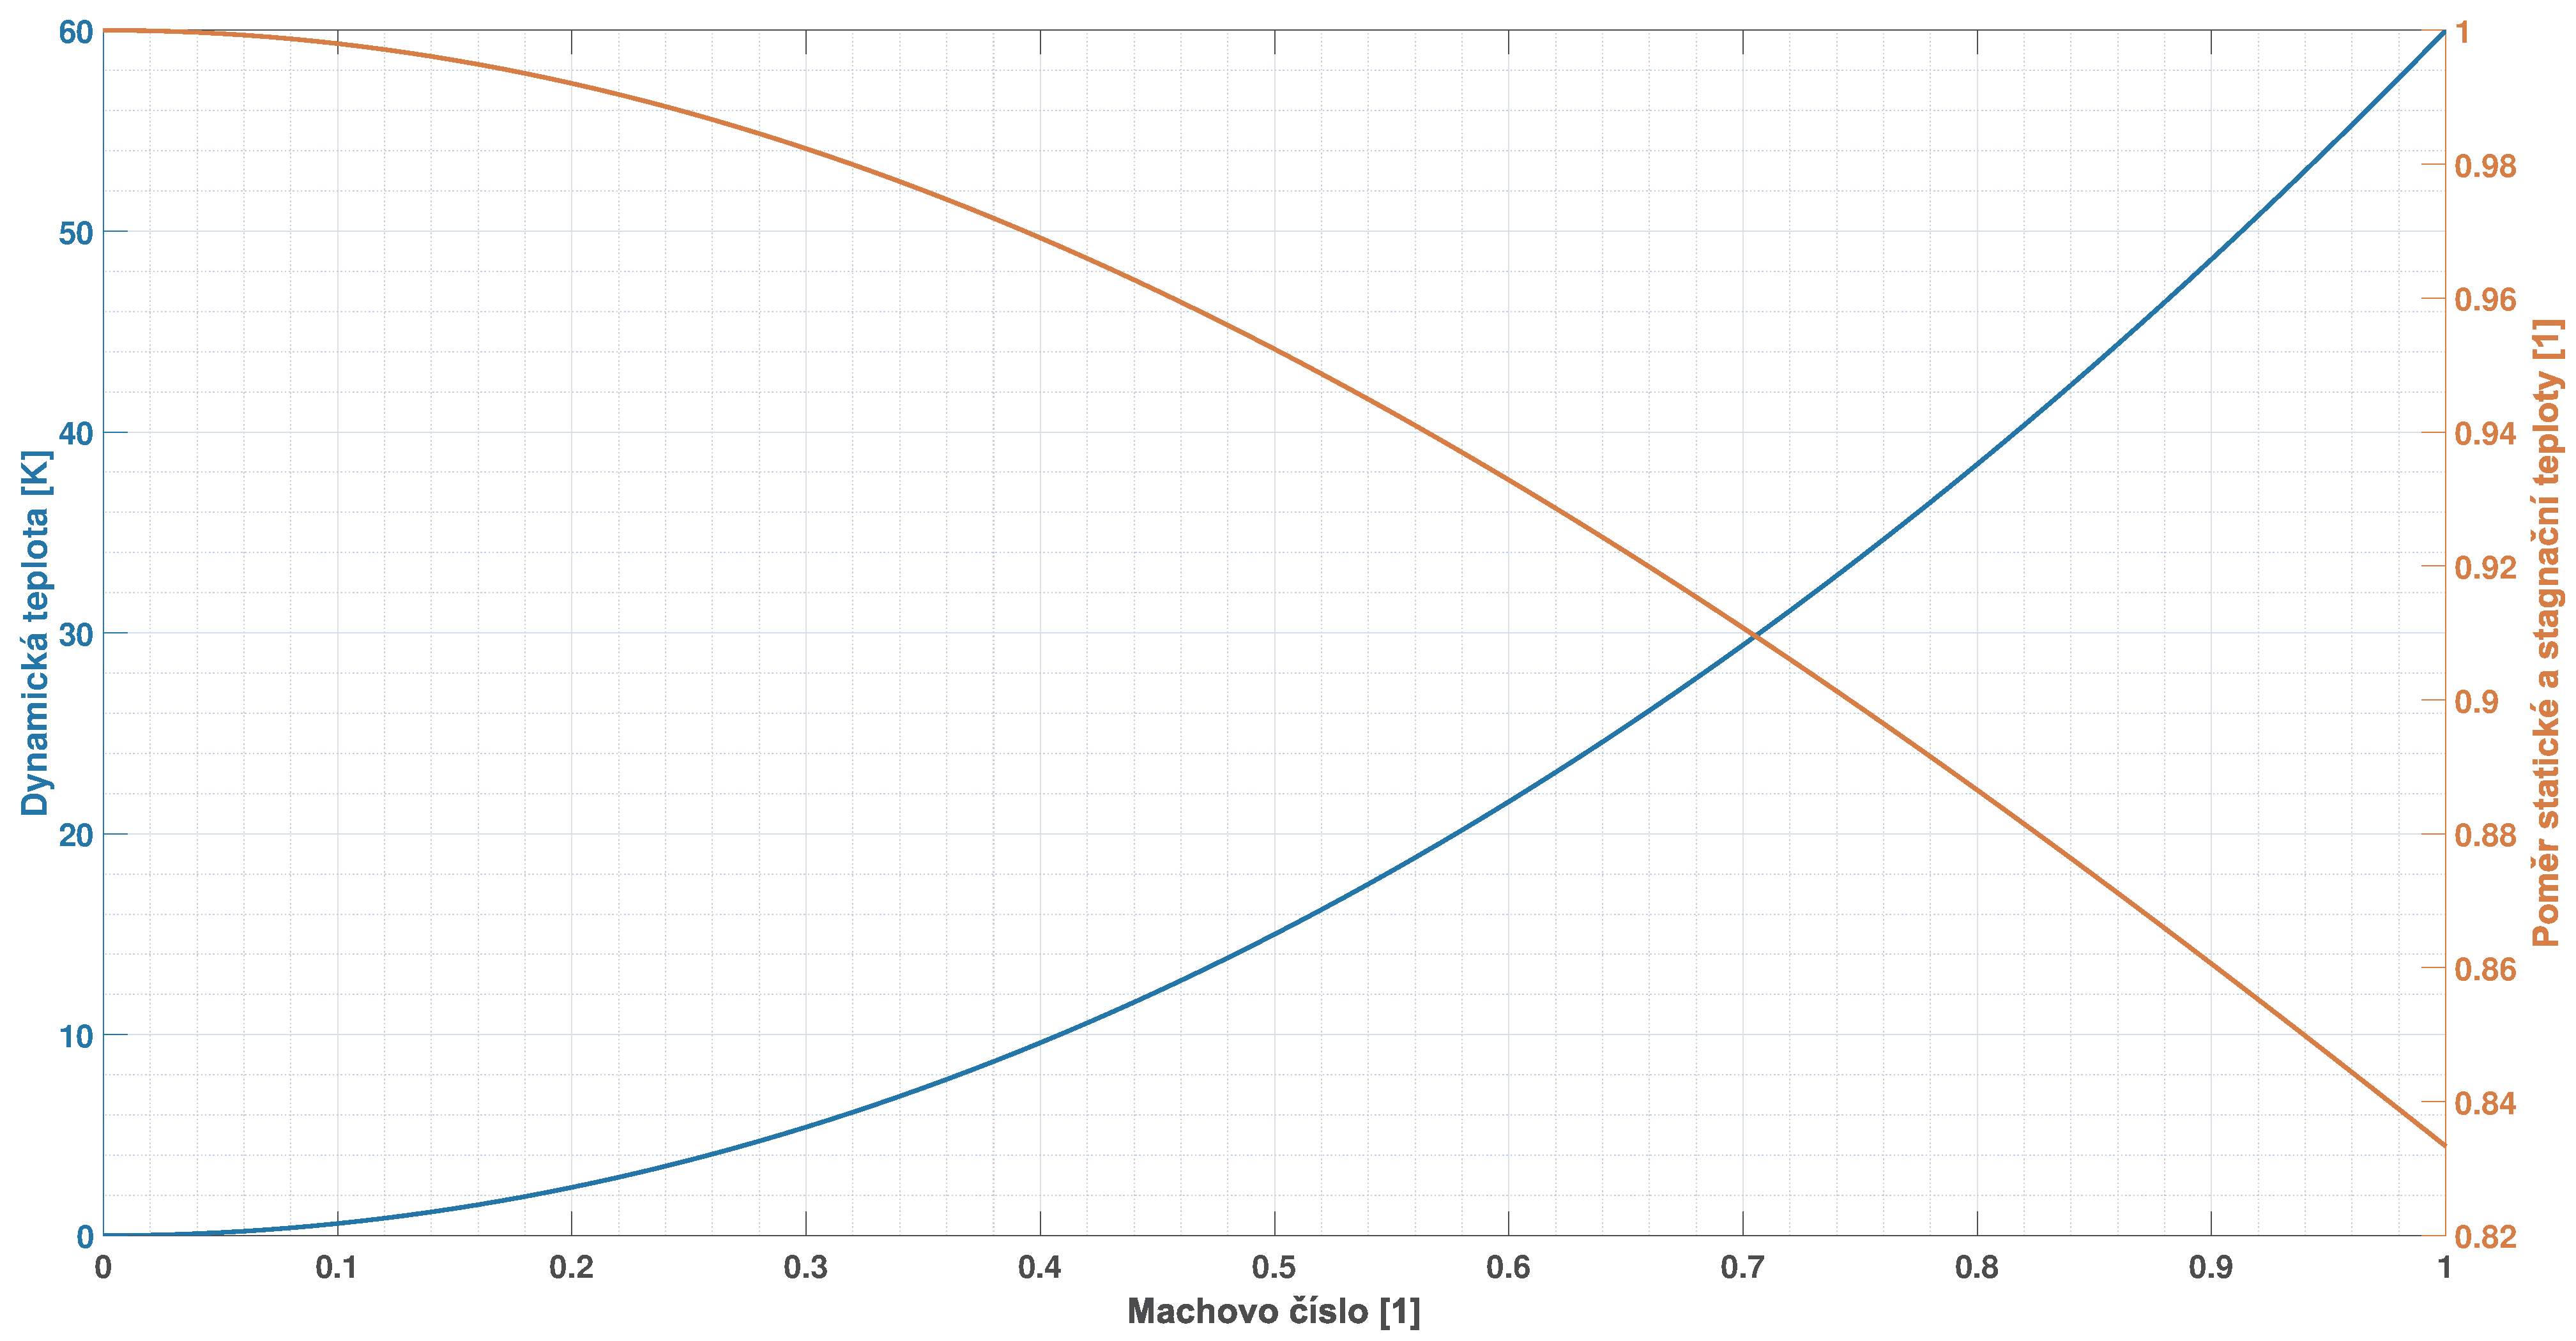
\includegraphics[width=\textwidth]{100_MERENI_TEPLOT/pomer_T_T0.eps}
        \caption{Závislost dynamické teploty a poměru $\frac{T}{T_0}$ na Machově čísle proudění pro statickou teplotu $300 \Unit{K}$.}
        \label{fig:pomer-T-T0}
    \end{figure}

    \subsection{Restituční faktor}

    Umístěním tělesa do proudu vzduchu dojde k jeho zahřívání vlivem zbrzdění proudění v mezní vrstvě. Budeme-li o tomto tělesu dále hovořit jako o teplotním snímači, tak bude klíčové, jakou teplotu naměříme. Ve stagnačním bodě snímače bude plyn dosahovat klidové teploty, mimo něj však bude teplota nižší. Měřená teplota, značená obvykle jako rovnovážná $T_r$, se tak bude pohybovat mezi teplotou statickou a stagnační ($T < T_r < T_0$). Vztah mezi těmito teplotami popisuje takzvaný restituční faktor $f$:
    \begin{equation} \label{eq:restitucni-faktor}
        f = \frac{T_r - T}{T_0 - T}
    \end{equation}

    Restituční faktor je především funkcí Prandtlova čísla, závisí však i na geometrii snímače a na Machově a Reynoldsově čísle \cite{Leontiev2017a}. Jeho hodnota je tedy proměnlivá, nicméně v řadě aplikací jej lze pro definované podmínky považovat za konstantu: pro válcová tělesa umístěná rovnoběžně v proudu vzduchu je při lokálním $\textrm{Re} < 5 \cdot 10^5$ restituční faktor roven $\sqrt{\textrm{Pr}}$, pro vzduch byla tato hodnota při $\textrm{Pr} = 0.72$ rovna $0.85$ \cite{Shapiro1954}. Obdobná hodnota restitučního faktoru (v tomto případě pro $\textrm{Pr}=0.71$) byla použita s dostatečnou přesností při měření pomocí termočlánku \cite{Ishibashi2012}.

    \subsection{Měření stagnační teploty}

    Kombinací Vztahů \ref{eq:restitucni-faktor} a \ref{eq:T0} lze získat vztahy pro výpočet rovnovážné teploty:
    \begin{align}
        f &= \frac{T_r - T}{T + \frac{u^2}{2 c_p} - T} \\
        T_r &= T + f \frac{u^2}{2 c_p} \\
        T_r &= T \brac{1 + f \frac{\kappa - 1}{2} \Ma ^2}
    \end{align}